\documentclass{report}

\usepackage{textcomp}
\usepackage{graphicx}
\usepackage{fancyhdr}
\usepackage{subcaption}
\usepackage{multicol}
\usepackage{outlines}
%===================================
\newcommand{\classinfo}{{\bf Troubleshooting Standard \\ IPV4 ACLs}\\{\it CIT 167 \\ Chaz Davis}}
\newcommand{\semester}{BCTC \\ Spring 2020}
%===================================
\newcommand{\mysection}[1]{\section*{#1}}
\newcommand{\mysubsection}[2]{\textbf{\romannumeral #1) #2}}
%===================================
\setlength{\headheight}{15.2pt}
\pagestyle{fancy}
\fancyhf{}
\lhead{ \fancyplain{}{Chaz Davis} }
\rhead{ \fancyplain{}{\today} }
\cfoot{ \fancyplain{}{\thepage} }
\renewcommand{\headrulewidth}{0.5pt}
\renewcommand{\footrulewidth}{0pt}

%===================================
\title{\classinfo}
\author{\semester}
\date{\today}

%===================================

\begin{document}

\maketitle

%===================================
\mysection{\textbf{Part 1: Troubleshoot ACL Issue 1}}

\mysubsection{1}{Determine ACL problem}\\
I realized that the Switches were misconfigured and had to reconnect them to
the correct interfaces on the routers.


Now, the first step is to check if LAN1 is denied access to LAN2,
so from L1 I will ping Server2. The successful output of that is in
Fig.~\ref{P1Net16}\subref{P1Net16Ping1} on Pg.~\pageref{P1Net16}. 


We are also told that Lan3 should have access to Lan2, so 
from L3 I will ping Server2. The ping was blocked by the router
,see Fig.~\ref{P1Net16}\subref{P1Net16Ping2} on Pg.~\pageref{P1Net16}.
Which means that Lan1 has access to Lan2 and Lan3 is blocked from Lan3. 


\begin{figure}[!hbt]\centering
\subfloat[L1 Pinging Server2]{\label{P1Net16Ping1}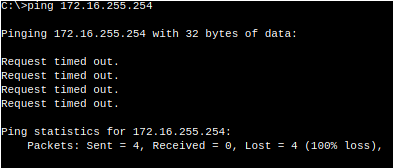
\includegraphics[width=.45\linewidth]{Figures/P1/L1Ping1.png}}\hfill
\subfloat[L3 Pinging Server2]{\label{P1Net16Ping2}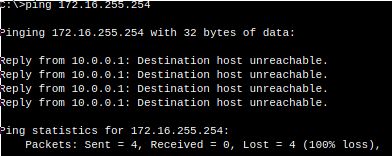
\includegraphics[width=.45\linewidth]{Figures/P1/L3Ping1.png}}\par 
\caption{Assessing the Network configs for DENY-LAN1 on R1}\label{P1Net16}
\end{figure}


\noindent\mysubsection{2}{Implement a Solution}\\
I logged into R1, I looked up the access tables, I went to
{\scriptsize{\verb$int g0/1$}\normalsize} and ran
{\scriptsize{\verb$no ip access-group DENY-LAN1 out$}\normalsize}. I then
reconfigured DENY-LAN1 to say 
{\scriptsize{\verb$20 permit any any$}\normalsize} that way it would 
allow all other addresses.  I then went to 
{\scriptsize{\verb$int g0/1$}\normalsize} and typed
in {\scriptsize{\verb$ip access-group DENY-LAN1 in$}\normalsize}. See
Fig.~\ref{P1Config16} on Pg.~\pageref{P1Config16} for outputs.


\begin{figure}[!hbt]\centering
\subfloat[Configuring the ACL DENY-LAN1]{\label{P1Config16Deny1}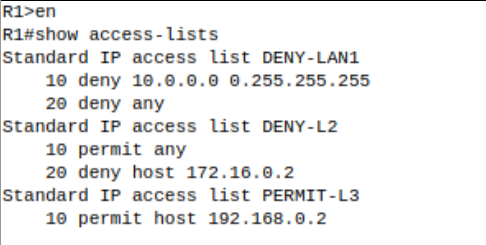
\includegraphics[width=.45\linewidth]{Figures/P1/Deny1.png}}\hfill
\subfloat[Output of the Access-lists]{\label{P1Config16Deny2}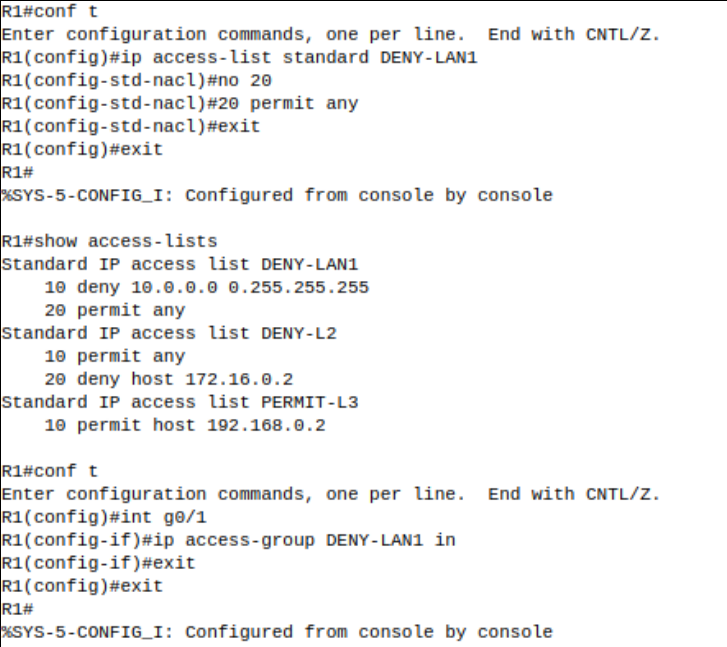
\includegraphics[width=.45\linewidth]{Figures/P1/Deny2.png}}\par 
\subfloat[G0/1 Configured with DENY-LAN1]{\label{P1Config16Deny3}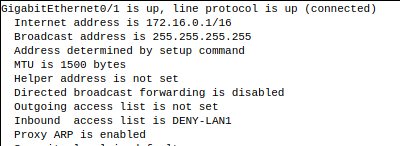
\includegraphics[width=.45\linewidth]{Figures/P1/Deny3.png}}
\caption{Configuring the ACL for R1 DENY-LAN1}\label{P1Config16}
\end{figure}



\noindent\mysubsection{3}{Verify that the problem is resolved and document the
solution}\\
I Verified the network connections by running a ping from L1 to
Server2(Fig.~\ref{P1Verify16}\subref{P1Verify16L1}), and
again from L3 to Server2(Fig.~\ref{P1Verify16}\subref{P1Verify16L3}).


\begin{figure}[!hbt]\centering
\subfloat[L1 Ping to Server2]{\label{P1Verify16L1}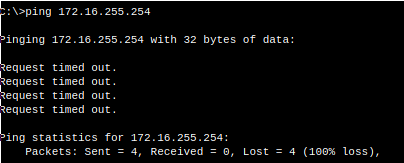
\includegraphics[width=.45\linewidth]{Figures/P1/L1Ping2.png}}\hfill
\subfloat[L3 Ping to Server2]{\label{P1Verify16L3}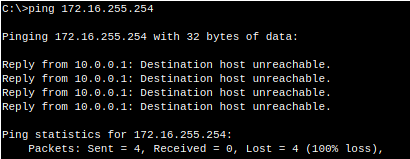
\includegraphics[width=.45\linewidth]{Figures/P1/L3Ping2.png}}\par 
\caption{Verifying DENY-LAN1 Connections}\label{P1Verify16}
\end{figure}


\clearpage

%===================================
\mysection{\textbf{Part 2: Troubleshoot ACL Issue 2}}


\mysubsection{1}{Determine the ACL problem}\\
The second thing we are told is that L2 should have access to LAN3. But, that 
Lan2 shouldn't have access to Lan3.  So, I will ping Server3 from L2. 
Next, I will ping Server3 from Server2. Both were unsuccessful. See Fig.~\ref{P2Net16}\subref{P2Net16Ping1} 
and Fig.~\ref{P2Net16}\subref{P2Net16Ping2}
on Pg.~\pageref{P2Net16} for those outputs.


Lastly, I ran the commands to show the output of access lists, 
to see how DENY-L2 was configured. See Fig.~\ref{P1Net16}\subref{P2Net16R1}.


\begin{figure}[!hbt]\centering
\subfloat[Pinging Server3 from L2]{\label{P2Net16Ping1}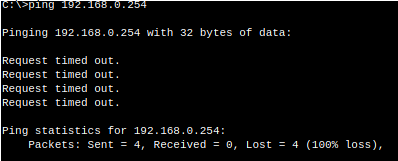
\includegraphics[width=.45\linewidth]{Figures/P2/L2Ping1.png}}\hfill
\subfloat[Pinging Server3 from Server2]{\label{P2Net16Ping2}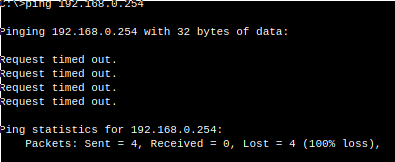
\includegraphics[width=.45\linewidth]{Figures/P2/Serv2Ping1.png}}\par 
\subfloat[DENY-L2 Access-list]{\label{P2Net16R1}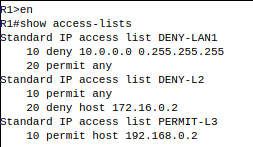
\includegraphics[width=.45\linewidth]{Figures/P2/R1config1.png}}
\caption{Determining the problems in part 2}\label{P2Net16}
\end{figure}

\noindent\mysubsection{2}{Implement a Solution}\\
I logged into R1, I looked up the access tables, I went to
{\scriptsize{\verb$int g0/2$}\normalsize} and ran
{\scriptsize{\verb$no ip access-group DENY-L2 out$}\normalsize}. I then
reconfigured DENY-L2 to say 
{\scriptsize{\verb$10 deny host 192.168.0.2$}\normalsize} 
{\scriptsize{\verb$20 permit any$}\normalsize} that way it would 
allow all other addresses.  I then went to 
{\scriptsize{\verb$int g0/1$}\normalsize} and typed
in {\scriptsize{\verb$ip access-group DENY-L2 in$}\normalsize}. See
Fig.~\ref{P2Config16} on Pg.~\pageref{P2Config16} for outputs.


\begin{figure}[!hbt]\centering
\subfloat[Configuring the ACL DENY-L2]{\label{P2Config16Deny1}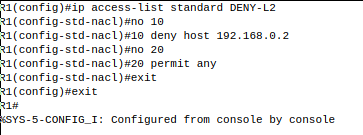
\includegraphics[width=.45\linewidth]{Figures/P2/Deny1.png}}\hfill
\subfloat[Output of the Access-lists]{\label{P2Config16Deny2}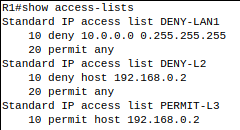
\includegraphics[width=.45\linewidth]{Figures/P2/Deny2.png}}\par 
\subfloat[G0/2 Configured with DENY-L2]{\label{P2Config16Deny3}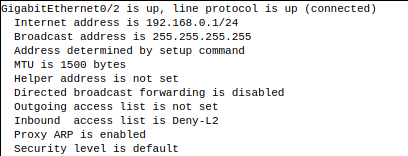
\includegraphics[width=.45\linewidth]{Figures/P2/Deny3.png}}
\caption{Configuring the ACL for R1 DENY-L2}\label{P2Config16}
\end{figure}


\noindent\mysubsection{3}{Verify that the problem is resolved and document the
solution}\\
I Verified the network connections by running a ping from L2 to
Server3(Fig.~\ref{P2Verify16}\subref{P2Verify16L2}), and
again from Server2 to Server3(Fig.~\ref{P2Verify16}\subref{P2Verify16Serv2}).


\begin{figure}[!hbt]\centering
\subfloat[L2 Ping to Server3]{\label{P2Verify16L2}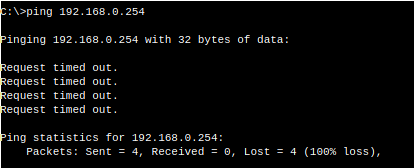
\includegraphics[width=.45\linewidth]{Figures/P2/L2Ping2.png}}\hfill
\subfloat[Server2 Ping to Server3]{\label{P2Verify16Serv2}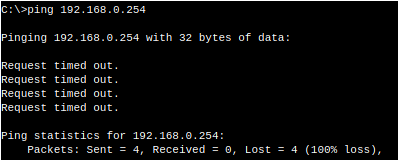
\includegraphics[width=.45\linewidth]{Figures/P2/Serv2Ping2.png}}\par 
\caption{Verifying DENY-L2 Connections}\label{P2Verify16}
\end{figure}


\clearpage


%===================================
\mysection{\textbf{Part 3: Troubleshoot ACL Issue 3}}


\mysubsection{1}{Determine the ACL problem}\\
Finally, we will test the connection to L1 and attempt to ping it both from L3, which
it should have access to, and then from server3, which should not have access
to it.
You can see in Fig.~\ref{P3Net16}~\subref{P3Net16Ping1} and
Fig.~\ref{P3Net16}\subref{P3Net16Ping2}
on Pg.~\pageref{P3Net16}.


\begin{figure}[!hbt]\centering
\subfloat[Pinging L1 from L3]{\label{P3Net16Ping1}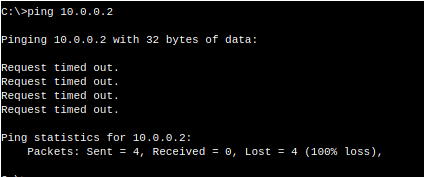
\includegraphics[width=.45\linewidth]{Figures/P3/L3PingL3.png}}\hfill
\subfloat[Pinging L1 from Server3]{\label{P3Net16Ping2}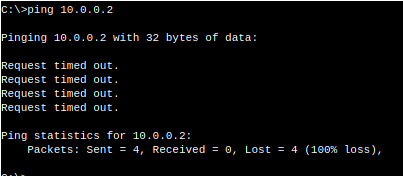
\includegraphics[width=.45\linewidth]{Figures/P3/Server3PingL1.png}}\par 
\subfloat[Show ip int of g0/0 for PERMIT-L3]{\label{P3Net16Show3}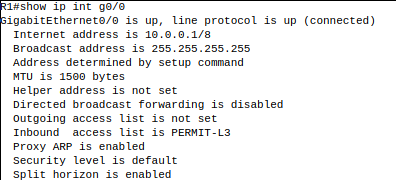
\includegraphics[width=.45\linewidth]{Figures/P3/Origconfigintg0-1.png}}
\caption{Checking original configuration of PERMIT-L3}\label{P3Net16}
\end{figure}



\noindent\mysubsection{2}{Implement a Solution}\\
To fix the problem, I changed the access-list from incoming to an outgoing
implementation. You can see in Fig.~\ref{P3Config16}~\subref{P3Confgi16a} 
on Pg.~\pageref{P3Config16}. 

We can now see the output of 
{\scriptsize{\verb$show access-lists$}\normalsize}
(Fig.~\ref{P3Config16}\subref{P3Config16b}) and 
{\scriptsize{\verb$show ip int$}\normalsize}
(Fig.~\ref{P3Config16}\subref{P3Config16c}).


\begin{figure}[!hbt]\centering
\subfloat[Configuring and applying
PERMIT-L3]{\label{P3Confgi16a}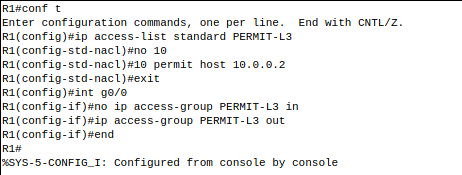
\includegraphics[width=.45\linewidth]{Figures/P3/cofigPermit-L3.png}}\hfill
\subfloat[show access-lists of
PERMIT-L3]{\label{P3Config16b}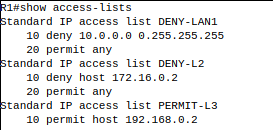
\includegraphics[width=.45\linewidth]{Figures/P3/ShowACL.png}}\par 
\subfloat[Show ip int of g0/0 with PERMIT-L3
applied]{\label{P3Config16c}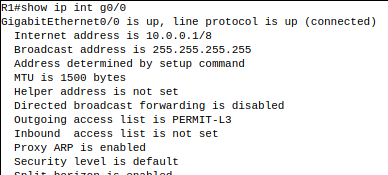
\includegraphics[width=.45\linewidth]{Figures/P3/showIPINT.png}}
\caption{Configuring PERMIT-L3}\label{P3Config16}
\end{figure}




\noindent\mysubsection{3}{Verify that the problem is resolved and document the
solution}\\
We can now see based off of the configurations we've implemented that the ping
from L3 to L1 is successful and that the ping from server3 to L1 is blocked at the router
(Fig.~\ref{P3Verify16}).


\begin{figure}[!hbt]\centering
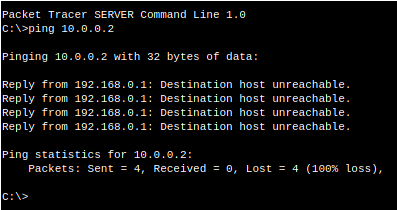
\includegraphics[width=.45\linewidth]{Figures/P3/Server3PinginL1.png}\par 
\caption{Server3 Blcoked pingin L1}\label{P3Verify16}
\end{figure}


\noindent{\bf{Wrap-up}}\\
We can now see  the ping's from each of the PC's to each of the servers,
Fig.~\ref{P3FinalP16}\subref{P3FinalP16a} through
Fig.~\ref{P3FinalP16}\subref{P3FinalP16c} on Pg.~\pageref{P3FinalP16}. 
We can see the final configurations of the interfaces,
Fig.~\ref{P3FinalC16}\subref{P3FinalC16a} through
Fig.~\ref{P3FinalC16}\subref{P3FinalC16c} on Pg.~\pageref{P3FinalC16}.
And we can see the completion of
activities, Fig.~\ref{P3FinalV16}\subref{P3FinalV16d} through
Fig.~\ref{P3FinalV16}\subref{P3FinalV16e} on Pg.~\pageref{P3FinalV16}.



\begin{figure}[!hbt]\centering
\subfloat[L1 Pinging Servers on the network]{\label{P3FinalP16a}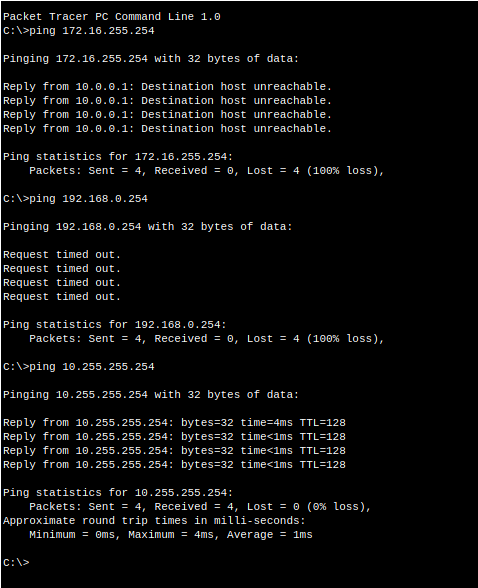
\includegraphics[width=.45\linewidth]{Figures/P3/L1PingingTheNet.png}}\hfill
\subfloat[L2 Pinging servers on the network]{\label{P3FinalP16b}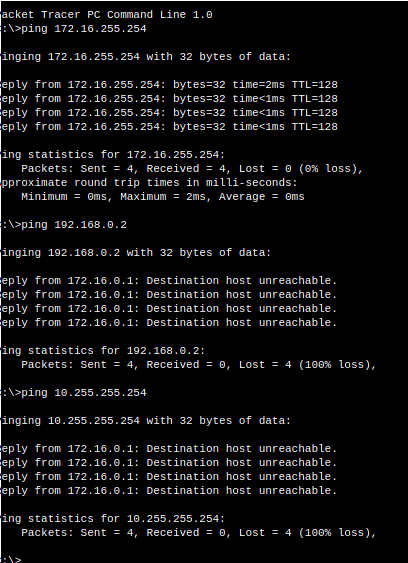
\includegraphics[width=.45\linewidth]{Figures/P3/L2PingingTheNet.png}}\par
\subfloat[L3 Pingin Servers on the network]{\label{P3FinalP16c}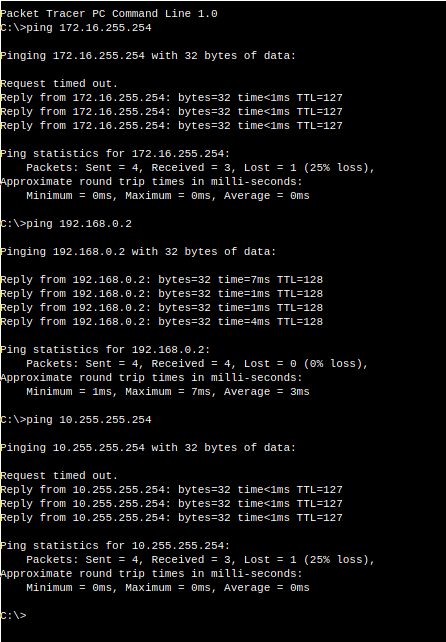
\includegraphics[width=.45\linewidth]{Figures/P3/L3PingingTheNet.png}}\par
\caption{Wrap-up and overview}\label{P3FinalP16}
\end{figure}

\begin{figure}[!hbt]\centering
\subfloat[Final Config of G0/0]{\label{P3FinalC16a}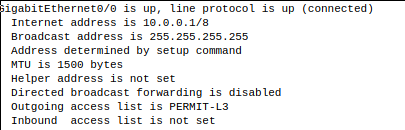
\includegraphics[width=.45\linewidth]{Figures/P3/showipintg0-1.png}}\hfill
\subfloat[Final Config for G0/1]{\label{P3FinalC16b}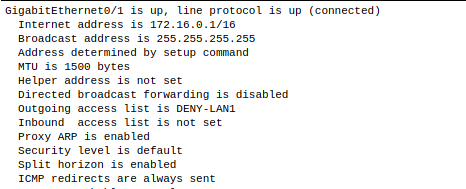
\includegraphics[width=.45\linewidth]{Figures/P3/showipintg1-1.png}}\par 
\subfloat[Final Config for G0/2]{\label{P3FinalC16c}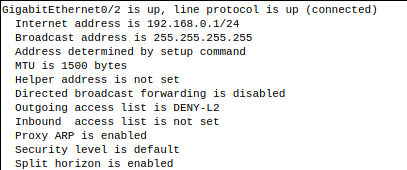
\includegraphics[width=.45\linewidth]{Figures/P3/showipintg2-1.png}}
\caption{Final Configuration for the network interfaces}\label{P3FinalC16}
\end{figure}


\begin{figure}[!hbt]\centering
\subfloat[Completion of activity]{\label{P3FinalV16d}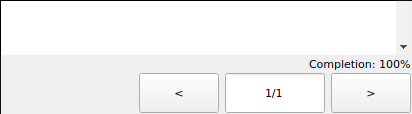
\includegraphics[width=.45\linewidth]{Figures/P3/Completion1.png}}\hfill
\subfloat[Completion of activity]{\label{P3FinalV16e}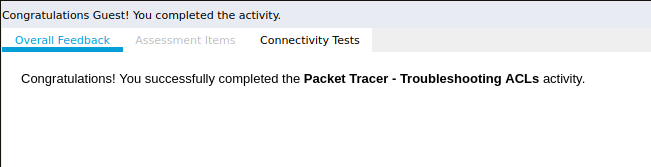
\includegraphics[width=.45\linewidth]{Figures/P3/Completion2.png}}\par
\caption{Completion of the Activity}\label{P3FinalV16}
\end{figure}




%===================================

\end{document}
